\documentclass[thesis]{subfiles}

\begin{document}

\chapter{Methodology}
\label{methodology}
% **************************** Define Graphics Path **************************
\ifpdf
    \graphicspath{{Figs/Raster/}{Figs/PDF/}{Figs/}}
\else
    \graphicspath{{Figs/Vector/}{Figs/}}
\fi

\section{Generalising Neural Networks and Decision Trees}
Although the relationship between neural networks and decision forests has been explored in the past, in the case of Entropy Nets~\cite{Sethi1990} this was with the intention of training and creating neural networks with decision-tree approaches, which restricts the representational ability of such networks to that of a decision tree. In the case of TODO...~\cite{Welbl2014casting}.

Here we explore the continuity of models between decision forests, with the objective of reducing the connectivity of deep neural networks trained with back-propagation, specifically convolutional neural networks, while retaining some of the efficiency and understanding which arise from the conditional computation in decision forests.

Towards this objective, we generalize neural networks and decision trees intuitively by using a new graphical notation for representing both. This notation isolates the differences between the two models, such that we can represent a hybrid model, \ie a \emph{Conditional Network}, compactly\footnote{This notation itself was created by Dr. Antonio Criminisi, and is not a contribution of this thesis. Some figures used with the permission of Dr. Antonio Criminisi/Microsoft Research.}.

\section{A New Graphical Notation}
The proposals we will make require a re-interpretation of existing classification models, that is neural networks and decision trees, but standard notation for both of these models hides the implicit functional similarities on which we will build our models. As such, before we are able to explain the concept of a conditional network, a new graphical language is proposed.

\subsection{Neural Networks}
\begin{figure}[htbp!] 
\centering
\begin{subfigure}[b]{0.45\textwidth}
   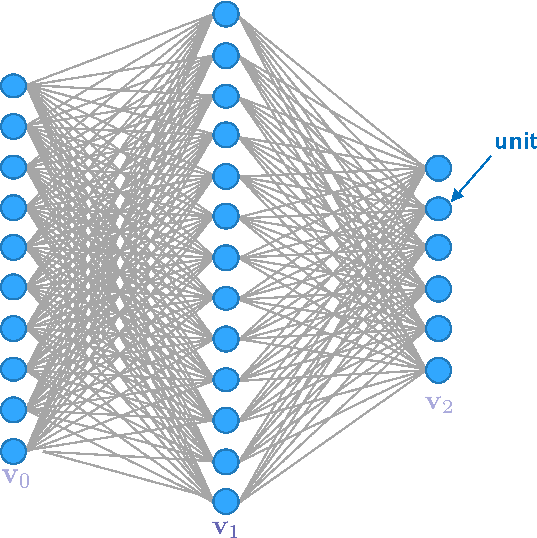
\includegraphics[width=\textwidth]{fullyconnected}
   \caption{Standard diagram of a neural network with one hidden layer.}
   \label{fig:oldnotation}
\end{subfigure}
~
\begin{subfigure}[b]{0.4\textwidth}
   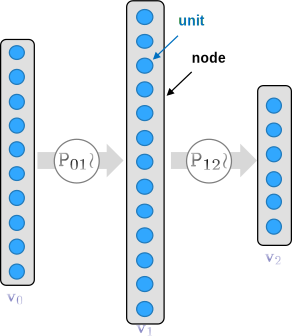
\includegraphics[width=\textwidth]{newnotation}
   \caption{New notation showing transformation between layers explicitly.}
   \label{fig:newnotation}
\end{subfigure}
\caption[New graphical notation for a standard neural network with one hidden layer.]{{\bf The proposed compact graphical notation for neural networks}. Non-linear transformations in a standard neural network with one hidden layer are indicated by the projection matrix $\mat P$ between the two layers, followed by a generic non-linearity, represented with the symbol $\wr$. Figures used with permission~\copyright Antonio Criminisi}
\label{fig:newGraphLanguage}
\end{figure}

The standard depiction of a neural network with one hidden layer is shown in Fig.~\ref{fig:oldnotation}, where each of the layers is fully connected, and these connecting weights are illustrated as lines between the neurons represented as circles. While this image illustrates the connectivity of the model, it assumes the function of the neurons themselves to be known or otherwise described. In Fig.~\ref{fig:newnotation}\ we use a different notation to show both connectivity and function of each layer, with the assumption that all nodes on a particular layer have the same function.

In this simple example of a fully-connected neural network, between layers $i$ and $j$, every node outputs the non-linear transformation, $\vec v_j = \sigma(\mat P \vec v_i)$, a composition of the non-linear function $\sigma$ (\eg a ReLU or sigmoid) and the projection of the input units with a projection matrix $\mat P$, which includes the bias term in homogeneous coordinates. We denote this operation explicitly as $\mat P_{ij} \wr$, where $\mat P_{ij}$ is the projection matrix and $\wr$ represents a non-linearity. In short $\mat P_{ij} \wr$ denotes the standard neural net layer's non-linear transformation $\vec v_j = \sigma(\mat P \vec v_i)$. 

Convolutional neural networks (CNNs) typical include layers with pooling operations (\eg max pooling), or local response normalization. Any of these operations may also be represented by the function $\sigma$.

\subsection{Decision Trees}
\begin{figure}[htbp!] 
\centering
\begin{subfigure}[b]{0.45\textwidth}
%   \includegraphics[width=\textwidth]{decisiontree}
   \caption{Standard diagram of a binary decision tree.}
   %\label{fig:oldtreenotation}
\end{subfigure}
~
\begin{subfigure}[b]{0.4\textwidth}
%   \includegraphics[width=\textwidth]{newdecisiontree}
   \caption{New notation showing transformation between levels explicitly.}
   %\label{fig:newtreenotation}
\end{subfigure}
\caption[New graphical notation for a binary decision tree.]{{\bf The proposed compact graphical notation for a decision tree}. \copyright Antonio Criminisi}
\label{fig:decisionTree}
\end{figure}

This graphical language may also represent decision trees. Decision trees typically copy, or reference, samples from the root of the tree down to the leaf (or leaves) without transformation. This may also be considered as a special case of the transformation $\vec v_j = \sigma(\mat P \vec v_i)$, where the projection is the identity matrix $\mat P_{ij} = \mat I$, and the function $\sigma$ is the identity function $\sigma(\vec v_i) = \vec v_i$. As such, we use the identity $\mat I$ in our graphical language to denote the routing between each tree level. 

We are still missing the method of conditional computation in our graphical language however, \ie how the decision is made to route each sample at a node. We must generalize two forms of routing found in decision trees, \emph{hard routing} where samples are only routed to one node in the next layer, and \emph{soft routing} where a weighted sample is potentially sent to every node of the next layer.

We achieve this with the minor addition of a new set of nodes we call a \emph{router}. A router consists of $K$ weights for a $K$-ary tree. These router weights themselves are determined in a way more reminiscent of a neuron's activation function, typically a non-linear transformation of the sample. Thus this is represented in the same graphical notation as the mapping between neural network layers, \ie as $\mat P_{ij} \wr$.

\end{document}